\documentclass[../main.tex]{subfiles}
	% INTRODUCTION
\begin{document}

This is what is going on over here.

%%%%%%%%%%%%%%%%%%%%%%%%%%%%%%%%%%%%%%%%%%%%%%%%%%%%%%%%%%%%%%%%%%%%%%%%%%%%%%%%%%%%%%%%%%%%%%%%%%%%%%%%%%%%%%%%%%%%%%%%%%%%%%%%%%

\todo[inline,color=green!40]{Figure out how the Intro Chapter will be formatted}
\section{Motivation}
Modern digital communication systems are built upon a solid foundation of modulation and coding theory.
Over the years, researchers have successfully developed numerous schemes using pen and paper along with computer models.
Any such scheme ultimately must be tested on a suitable hardware/software platform to prove their usefulness in practice.
Standard ‘software-defined radio’ test beds can cost thousands of pounds.
Although these test beds provide users with advanced development tools, much of their functionality is superfluous to requirement.\\

A Raspberry Pi is a simple, affordable ARM-based computer module that is capable of interfacing with external peripheral devices through a bank of IO ports.
It is also programmable (using Python), and as such has found many uses by hobbyists and electronics/computer engineers in recent years.
The purpose of this project is to develop a basic digital communication test bed using two Raspberry Pi modules (one transmitter and one receiver).
The test bed will be affordable and the interested student will need to work to a budget to ensure a successful outcome.
The project will require a considerable amount of Python programming as well as knowledge of, and a keen interest in, digital communication theory and techniques.

%%%%%%%%%%%%%%%%%%%%%%%%%%%%%%%%%%%%%%%%%%%%%%%%%%%%%%%%%%%%%%%%%%%%%%%%%%%%%%%%%%%%%%%%%%%%%%%%%%%%%%%%%%%%%%%%%%%%%%%%%%%%%%%%%%

\section{Background - Literature Review}
Explanation of the existing literature \cite{DhirNIPS2017}.

\begin{figure}[ht]
	\centering
	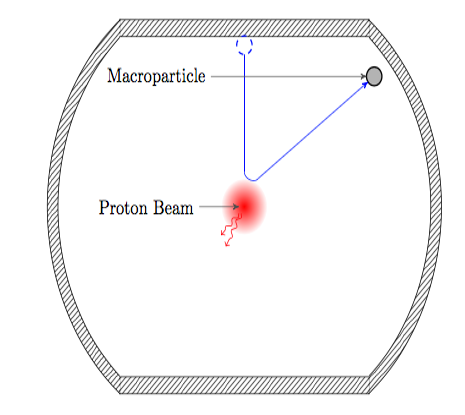
\includegraphics[width=0.4\textwidth]{UFO_Falling.png}
	\caption{UFO Depicted Falling into the Proton Beam}
	%\label{}
\end{figure}

Chat chat chat.

\begin{equation} \label{bla}
\textbf{F}(t) = (\textbf{m}(t)\cdot\nabla)\textbf{E}(t)
\end{equation}

where $\textbf{E}(t)$ is the electric field in \SI{150}{\centi \tesla}.

%%%%%%%%%%%%%%%%%%%%%%%%%%%%%%%%%%%%%%%%%%%%%%%%%%%%%%%%%%%%%%%%%%%%%%%%%%%%%%%%%%%%%%%%%%%%%%%%%%%%%%%%%%%%%%%%%%%%%%%%%%%%%%%%%%

\section{(My) Contributions}

\end{document}  